\documentclass{jarticle}
\usepackage[dvipdfmx]{graphicx}
\usepackage{here}
\usepackage{listings,jlisting}


\lstset{
  basicstyle={\ttfamily},
  identifierstyle={\small},
  commentstyle={\smallitshape},
  keywordstyle={\small\bfseries},
  ndkeywordstyle={\small},
  stringstyle={\small\ttfamily},
  frame={tb},
  breaklines=true,
  columns=[l]{fullflexible},
  numbers=left,
  xrightmargin=0zw,
  xleftmargin=3zw,
  numberstyle={\scriptsize},
  stepnumber=1,
  numbersep=1zw,
  lineskip=-0.5ex
}

\title{{システム実験}\\実験6回レポート}
\author{6119019056 山口力也}
\date{2019/05/31日提出}

\begin{document}
\maketitle

\section{ArduinoからProcessingへのデータ送信:通信方式1}
演習3.1.7の5で考察した内容を報告せよ.

フレームレートの値を大きくすると,描画の頻度が増える.しかしながら,データ受信のタイミングより早くなると描画が間に合わなくなるので逆に遅延が発生した.フレームレートの値を小さくすると描画のタイミングが遅いので,半固定抵抗を素早く上下させたときの値が読み取れていなかった.

\section{ArduinoからProcessingへのデータ送信:通信方式2}
演習3.1.8の5で考察した内容を報告せよ.
ハンドシェイクで通信を行うと,描画とデータ受信が常に交互に行われていた.コネクションが確立されてから通信を行うためだと考えられる.ハンドシェイク(3-way handshaking)について調べると,TCP/IPでも使われているようだった.
\section{繰り返し処理による描画(2Dバージョン)}
課題3.1.1で作成したスケッチ(draw\_latice\_2D)を報告せよ.

以下ソースコード\ref{code:kadai3-1-1}にスケッチを示す.

\begin{lstlisting}[caption = 課題3.1.1,label=code:kadai3-1-1][H]
int xn = 10; //x軸の格子
int yn = 10; //y軸の格子


int x,y; //x座標とy座標を定義

size(600,600); //ウィンドウサイズ600*600
background(255); //背景白

stroke(0); //線の色黒
for(int i =0; i<=yn; i++){ //格子の横線
  y =  i*height/yn; //線のy座標
  line(0,y,width,y); //線を描画
}

for(int i = 0; i<= xn; i++){ //格子の縦線
  x = i*width/xn; //線のx座標
  line(x,0,x,height); //線を描画
}

stroke(255,0,0);
for(int i_c =0; i_c<xn; i_c++){ //i_cはマス目のインデックス
  for(int i_r = 0; i_r < yn; i_r++){
    x = width/(2*xn) + i_c*width/xn; //30 + 60*i_c
    y = height/(2*yn) + i_r*height/yn; //30 + 60*i_r
    ellipse(x,y,width/xn,height/yn); //円を描画
  }
}
\end{lstlisting}

\section{動画の作成:移動する楕円(2Dバージョン)}
課題3.1.2で作成したスケッチ(draw\_latice\_2D)を報告せよ.

以下ソースコード\ref{code:kadai3-1-2}にスケッチを示す.

\begin{lstlisting}[caption = 課題3.1.2,label=code:kadai3-1-2][H]
int xn = 10; //分割数
int yn = 10; //分割数
int i_c; //楕円を描くマス目番号
int i_r; //楕円を描くマス目番号
int flag_upper_right = 0; //右上端フラグ
int flag_upper_left = 0; //左上端フラグ
int flag_down_right =0; //右下端フラグ
int flag_down_left = 0; //左下端フラグ

void setup(){
  size(600,600); //ウィンドウサイズ600*600
  frameRate(20); //フレームレート20
  i_c = 0; //列
  i_r = 0; //行
}
void draw()
{
  int x,y; //x座標とy座標
  background(255); //背景白
  stroke(0); //線の色黒
  for(int i = 0; i<= yn; i++){
    y =  i*height/yn; //線のy座標
    line(0,y,width,y);
  }
  for(int i = 0; i<= xn; i++){ //格子の縦線
    x = i*width/xn; //線のx座標
    line(x,0,x,height);
  }
  stroke(255,0,0);
  x = width/(2*xn) + i_c*width/xn; //30 + 60*i_c
  y = height/(2*yn) + i_r*height/yn; //30 + 60*i_r
  ellipse(x,y,width/xn,height/yn);
  //楕円を描くマス目番号の更新
  if ( i_c == 0 && i_r == 0){ //左上端の時
    flag_upper_left = 1;
    flag_upper_right = 0;
    flag_down_left = 0 ;
    flag_down_right = 0;
    println("upperleftnow");
  }
  if ( i_c == xn-1 && i_r == 0){ //右上端の時
    flag_upper_left = 0;
    flag_upper_right = 1;
    flag_down_left = 0 ;
    flag_down_right = 0;
    println("upperrightnow");
  }
  if ( i_c == 0 && i_r == yn-1){ //左下端の時

    flag_upper_left = 0;
    flag_upper_right = 0;
    flag_down_left = 1 ;
    flag_down_right = 0;
    println("downleftnow");
  }
  if ( i_c == xn-1 && i_r == yn-1){ //右下端の時

    flag_upper_left = 0;
    flag_upper_right = 0;
    flag_down_left = 0 ;
    flag_down_right = 1;
    println("downrightnow");
  }
  if(flag_upper_left == 1){
    i_c++;
  }
  if(flag_upper_right == 1){
    i_c--;
    i_r++;
  }
  if(flag_down_left == 1){
    i_c++;
  }
  if(flag_down_right == 1){
    i_c--;
    i_r--;
  }
  
}
\end{lstlisting}

\section{電圧変化の時間軸グラフによる可視化(点のプロット)}
課題3.1.3で作成したProcessingのスケッチを報告せよ.また,出力したウィンドウのスナップショットを報告せよ.
以下ソースコード\ref{code:kadai3-1-3}にスケッチを示す.

\begin{lstlisting}[caption = 課題3.1.3,label=code:kadai3-1-3][H]
import processing.serial.*; // Serial ライブラリを取り込む
Serial port; // Serial クラスのオブジェクトを宣言
int val,count,x,y; //変数宣言
void setup()
{
  size(800,300); // サイズ 800 × 300 のウィンドウ生成
  port = new Serial(this, "/dev/ttyACM0", 9600);//Serial クラスのインスタンス生成
  val = 0;
  count = 0;
  x = 0;
  y = 0;
  background(255); //背景白 
}
void draw()
{
  stroke(255,0,0); //赤色
  strokeWeight(5); //太さを5
  x = count; //countを代入
  y = (255 - val)*300/255; //val=0で300,val=255で0
  point(x,y); //点を描画
  if( count == 800){ //右端についたら
    count = 0; //初期化
    background(255); //背景をクリア 
  }
  println("R"); // 描画タイミング(確認用)
}
// シリアルポートにデータが到着するたびに呼び出される割り込み関数
void serialEvent(Serial p) { // p にはデータが到着したシリアルポートに対応するインスタンス(ここでは port )が代入される
  val = p.read(); // 受信バッファから 1 バイト読み込み
  println("<-");
  count++;
// データ受信タイミング(確認用)
}
\end{lstlisting}

また,以下図\ref{fig:kadai3-1-3}に出力したウィンドウのスナップショットを示す.

\begin{figure}[H]
\begin{center}
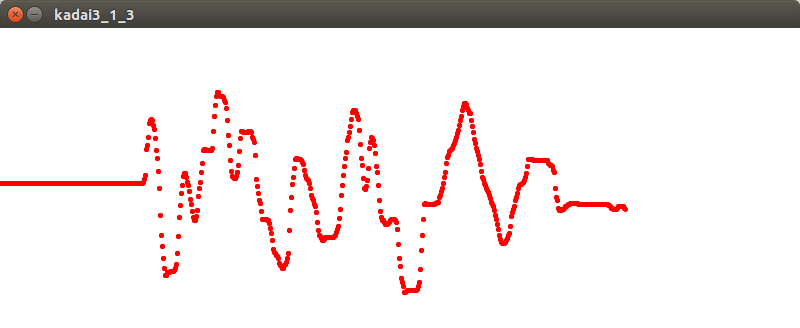
\includegraphics[width=7.0cm]{images/kadai3-1-3.png}
\caption{課題3.1.3の出力画像}
\label{fig:kadai3-1-3}
\end{center}
\end{figure}


\section{電圧変化の時間軸グラフによる可視化(折れ線)}
課題3.1.4で作成したProcessingのスケッチを報告せよ.また,出力したウィンドウのスナップショットを報告せよ.
以下ソースコード\ref{code:kadai3-1-4}にスケッチを示す.

\begin{lstlisting}[caption = 課題3.1.4,label=code:kadai3-1-4][H]
import processing.serial.*; // Serial ライブラリを取り込む
Serial port; // Serial クラスのオブジェクトを宣言
int val,count,new_x,new_y,old_x,old_y; //それぞれ値を定義
void setup()
{
  size(800,300); // サイズ 800 × 300 のウィンドウ生成
  port = new Serial(this, "/dev/ttyACM0", 9600);//Serial クラスのインスタンス生成
  val = 0; //Arduinoから送られてきたデータを格納する
  count = 0; //受信した回数(x座標)
  old_x = 0; //折れ線グラフ用の前回のxの値
  old_y = 0; //折れ線グラフ用の前回のyの値
  new_x = 0; //折れ線グラフ用の今のxの値
  new_y = 0; //折れ線グラフ用の今のyの値
  background(255); // 背景を白に設定
}
void draw()
{
  stroke(255,0,0); //線の色を赤に設定
  strokeWeight(5); //線の太さを"5"に設定
  new_x = count; //x座標の値はcountそのもの
  new_y = (255 - val)*300/255; //y座標の値はval=255のときy=0(一番上),val=0のときy=300(一番下)
  point(new_x,new_y); //点を描画
  strokeWeight(3); //線の太さを"3"に設定
  line(old_x,old_y,new_x,new_y); //折れ線用に線を描画
  old_x = new_x; //今のxの値を前回の値として格納
  old_y = new_y; //今のyの値を前回の値として格納
  if( count == 800){ //もし右端まできたら
    count = 0; //count初期化
    background(255); //背景を白に(クリア)
  }
  println("R"); // 描画タイミング(確認用)
}
// シリアルポートにデータが到着するたびに呼び出される割り込み関数
void serialEvent(Serial p) { // p にはデータが到着したシリアルポートに対応するインスタンス(ここでは port )が代入される
  val = p.read(); // 受信バッファから 1 バイト読み込み
  println("<-"); // データ受信タイミング(確認用)
  count++; //countを1増やす(x座標を1つ右にずらす)
}
\end{lstlisting}
また,以下図\ref{fig:kadai3-1-4}に出力したウィンドウのスナップショットを示す.

\begin{figure}[H]
\begin{center}
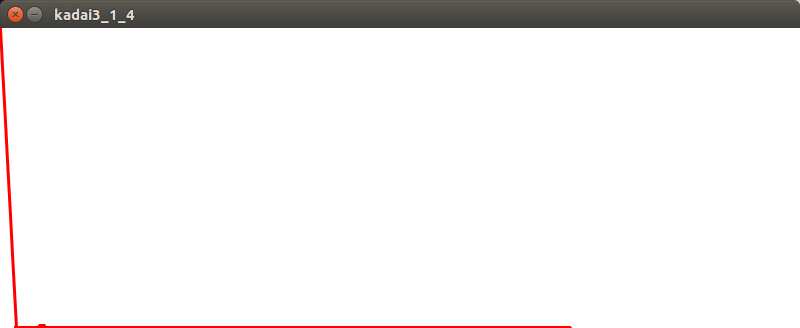
\includegraphics[width=7.0cm]{images/kadai3-1-4-2.png}
\caption{課題3.1.4の出力画像}
\label{fig:kadai3-1-4}
\end{center}
\end{figure}

照度センサの場合,図\ref{fig:kadai3-1-4}のように変化が分かりづらかったため半固定抵抗のスナップショットを以下図\ref{fig:kadai3-1-4-1}に示す.

\begin{figure}[H]
\begin{center}
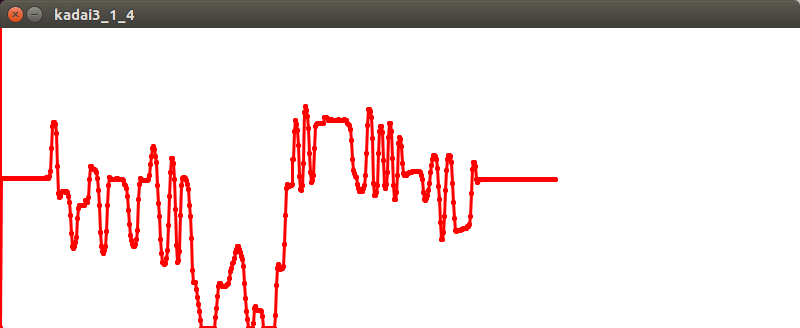
\includegraphics[width=7.0cm]{images/kadai3-1-4-1.png}
\caption{課題3.1.4の出力画像(半固定抵抗)}
\label{fig:kadai3-1-4-1}
\end{center}
\end{figure}


\section{電圧変化のメーター表示}
課題3.1.5で作成したProcessingのスケッチを報告せよ.また,出力したウィンドウのスナップショットを報告せよ.
以下ソースコード\ref{code:kadai3-1-5}にスケッチを示す.

\begin{lstlisting}[caption = 課題3.1.5,label=code:kadai3-1-5][H]
import processing.serial.*; // Serial ライブラリを取り込む
Serial port; // Serial クラスのオブジェクトを宣言
float rad,x,y; //ラジアン,x,yをそれぞれ定義
int val; //Arduinoから送られてくるデータ格納用

void setup()
{
  size(500,500); // サイズ 500 × 500 のウィンドウ生成
  port = new Serial(this, "/dev/ttyACM0", 9600);//Serial クラスのインスタンス生成

}
void draw()
{
  background(255); //背景を白に設定
  stroke(0,0,0); //線を黒に設定
  ellipse(200,200,200,200); //円を描画
  stroke(255,0,0); //線を赤に設定
  strokeWeight(5); //線の太さを"5"に設定
  rad = 2*PI*val/255; //受信したデータをラジアンに変換(255で2π,0で0)
  x = 200 + 100*cos(rad - PI/2); //x座標の値(中心200から距離cos(rad - π/2)
  y = 200 + 100*sin(rad - PI/2); //y座標の値(中心200から距離sin(rad - π/2)
  line(200,200,x,y); //メータの線を描画
  println("R"); // 描画タイミング(確認用)
}
// シリアルポートにデータが到着するたびに呼び出される割り込み関数
void serialEvent(Serial p) { // p にはデータが到着したシリアルポートに対応するインスタンス(ここでは port )が代入される
  val = p.read(); // 受信バッファから 1 バイト読み込み
  println("<-"); // データ受信タイミング(確認用)
}
\end{lstlisting}
また,以下図\ref{fig:kadai3-1-5}に出力したウィンドウのスナップショットを示す.

\begin{figure}[H]
\begin{center}
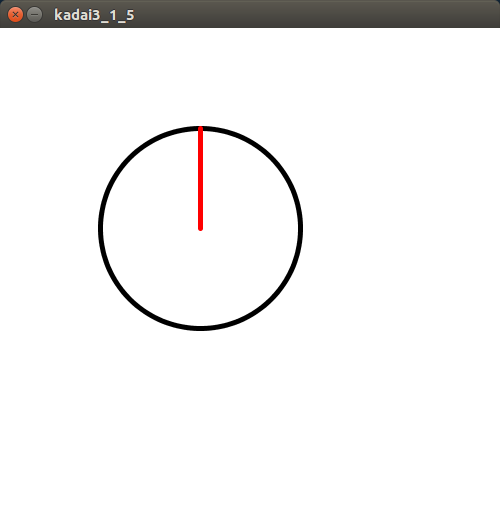
\includegraphics[width=7.0cm]{images/kadai3-1-5.png}
\caption{課題3.1.5の出力画像}
\label{fig:kadai3-1-5}
\end{center}
\end{figure}


\section{発展課題3.1.1 複数データの送信}
発展課題3.1.1で作成したArduinoとProcessingのスケッチを報告せよ.
以下ソースコード\ref{code:hatten3-1-1-a},\ref{code:hatten3-1-1-p}にそれぞれArduinoとProcessingのスケッチを示す.

\begin{lstlisting}[caption = 発展課題3.1.1(Arduino),label=code:hatten3-1-1-a][H]
int sensorValue1,sensorValue2,sendValue1,sendValue2;
unsigned long int timePrev, timeNow;
void setup()
{
  Serial.begin(9600); // シリアル通信を 9600bps で初期化
  timePrev = millis(); // 経過時間の初期値
}
void loop()
{
  timeNow = millis(); // 現在の経過時間
  sensorValue1 = analogRead(0); // A0 ピンの AD 変換結果を取得 (0-1023)
  sensorValue2 = analogRead(1); // A1 ピンの AD 変換結果を取得 (0-1023)
  if ( timeNow - timePrev >= 50 ) { // 50ms ごとに実行
    sendValue1 = sensorValue1 /4; // 0-255 の値に変換
    sendValue2 = sensorValue2 /4; // 0-255 の値に変換
    Serial.write('A');
    Serial.write(sendValue1); // 1 バイトのバイナリデータとして値を送信
    Serial.write(sendValue2); // 1 バイトのバイナリデータとして値を送信
    timePrev = timeNow; // 1 ステップ前の経過時間を更新
  }
}
\end{lstlisting}

\begin{lstlisting}[caption = 発展課題3.1.1(Processing),label=code:hatten3-1-1-p][H]
import processing.serial.*; // Serial ライブラリを取り込む
Serial port; // Serial クラスのオブジェクトを宣言
int val1,val2; //縦幅と横幅
void setup()
{
  size(256, 256); // サイズ 256 × 256 のウィンドウ生成
  port = new Serial(this, "/dev/ttyACM0", 9600);//Serial クラスのインスタンス生成
}
void draw()
{
  background(0); // 背景を黒
  ellipse(125, 125, val1, val2); // 中心 (125,125) ,横幅val1,縦幅val2 の円(白塗り)を描画
  println("R"); // 描画タイミング(確認用)
}
// シリアルポートにデータが到着するたびに呼び出される割り込み関数
void serialEvent(Serial p) { // p にはデータが到着したシリアルポートに対応するインスタンス(ここでは port )が代入される
  if(p.available() >= 3){
    if(p.read() == 'A'){ //識別子Aを定義
      val1 = p.read(); //読み込み
      val2 = p.read(); //読み込み
      p.clear();
      println("<-");  // データ受信タイミング(確認用)
      println("val1=",val1); //確認用
      println("val2=",val2); //確認用
    }
  }
}

\end{lstlisting}


また,以下図\ref{fig:hatten3-1-1}に出力したウィンドウのスナップショットを示す.

\begin{figure}[H]
\begin{center}
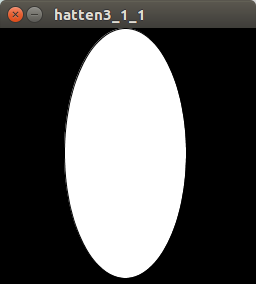
\includegraphics[width=7.0cm]{images/hatten3-1-1.png}
\caption{発展課題3.1.1の出力画像}
\label{fig:hatten3-1-1}
\end{center}
\end{figure}


\section{発展課題3.1.2 バーコレーションシミュレーション}
こちらは時間が足りずにできなかった.

\end{document}
